\documentclass[tikz,border=10pt]{standalone}
\usepackage{amsmath}
\usetikzlibrary{arrows.meta}
\definecolor{ink}{HTML}{21352F}
\definecolor{teal}{HTML}{087F7B}
\definecolor{blue}{HTML}{4B77A8}
\definecolor{gold}{HTML}{C58B2A}

\begin{document}
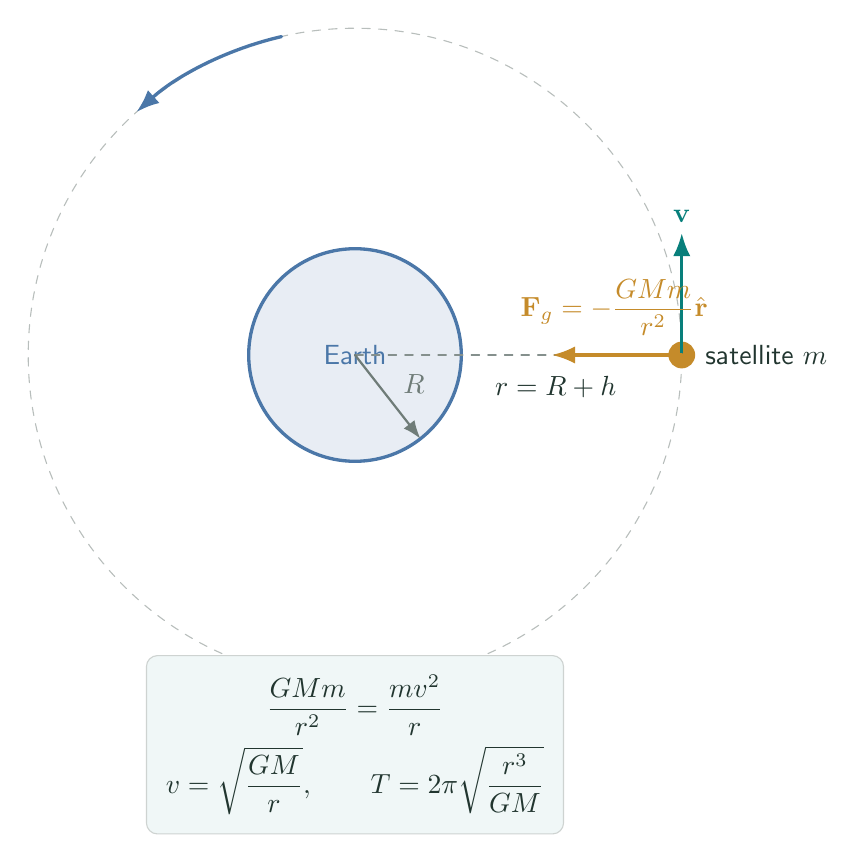
\begin{tikzpicture}[font=\sffamily,text=ink,>=Latex,line cap=round,line join=round]
  \def\earthradius{1.35}
  \def\orbitradius{4.15}
  \coordinate (O) at (0,0);
  \coordinate (S) at (0:\orbitradius);

  \fill[blue!13] (O) circle (\earthradius);
  \draw[blue,very thick] (O) circle (\earthradius);
  \node[blue] at (O) {Earth};

  \draw[ink!32,dashed] (O) circle (\orbitradius);
  \draw[blue,very thick,->]
    (103:\orbitradius) arc[start angle=103,end angle=132,radius=\orbitradius];

  \draw[ink!55,dashed] (O)--(S);
  \node[below=4pt] at (2.55,0) {$r=R+h$};
  \draw[ink!65,thick,->] (O)--(-52:\earthradius)
    node[pos=.58,above right] {$R$};

  \fill[gold] (S) circle (0.17);
  \node[right=5pt] at (S) {satellite $m$};
  \draw[teal,very thick,->] (S)--++(0,1.55)
    node[above] {$\mathbf v$};
  \draw[gold,very thick,->] (S)--++(-1.65,0)
    node[pos=.52,above=3pt] {$\displaystyle\mathbf F_g=-\frac{GMm}{r^2}\hat{\mathbf r}$};

  \node[draw=ink!22,rounded corners=4pt,fill=teal!6,align=center,
        inner sep=7pt] at (0,-4.95)
    {$\displaystyle \frac{GMm}{r^2}=\frac{mv^2}{r}$\\[3pt]
     $\displaystyle v=\sqrt{\frac{GM}{r}},\qquad
       T=2\pi\sqrt{\frac{r^3}{GM}}$};
\end{tikzpicture}
\end{document}
